\section{Extracción de características}\label{sec:features}

\begin{frame}
    \frametitle{Extracción de características}

    \begin{block}{Sonido}
        Variación en la presión que ejerce el medio que lo transmite sobre su receptor.
        \begin{itemize}
            \item<2-> \textbf{Frecuencia}: Cantidad de vibraciones por segundo (medida en Hertz).
            \item<3-> \textbf{Amplitud}: Intensidad de las vibraciones (medida arbitraria).
        \end{itemize}
    \end{block}

    \begin{itemize}
        \item<4-> \textit{Periódicos}.
        \begin{itemize}
            \item Período (en segundos)
            \item Frecuencia (en Hertz)
        \end{itemize}
        \item<5-> \textit{Armónicos}.
        \item<6-> \textit{Ruidos}.
    \end{itemize}
\end{frame}

\begin{frame}
    \frametitle{Extracción de características}

    \begin{columns}
        \column{0.5\textwidth}

        \begin{figure}[!h]
            \centering
            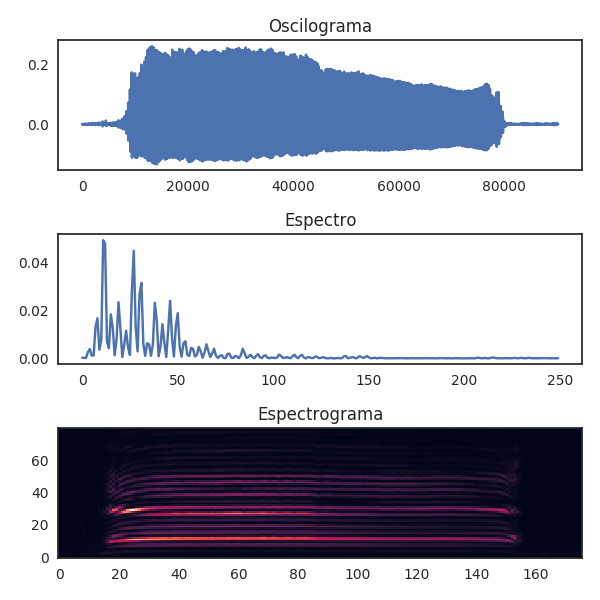
\includegraphics[width=\textwidth]{oscillogram+spectrum+spectrogram.png}
        \end{figure}

        \pause
        \column{0.5\textwidth}

        Pasos para la conversión de una señal del dominio analógico al digital:
        \begin{enumerate}
            \item<3-> \textbf{Filtrado} al intervalo de frecuencias $[0,B]$.
            \item<4-> \textbf{Muestreo} con frecuencia $F_s = 2B$.
            \item<5-> \textbf{Cuantificación}.
        \end{enumerate}

    \end{columns}
\end{frame}

\begin{frame}
    \frametitle{Características temporales}

    \begin{columns}
        \column{0.5\textwidth}

        \begin{figure}[!h]
            \centering
            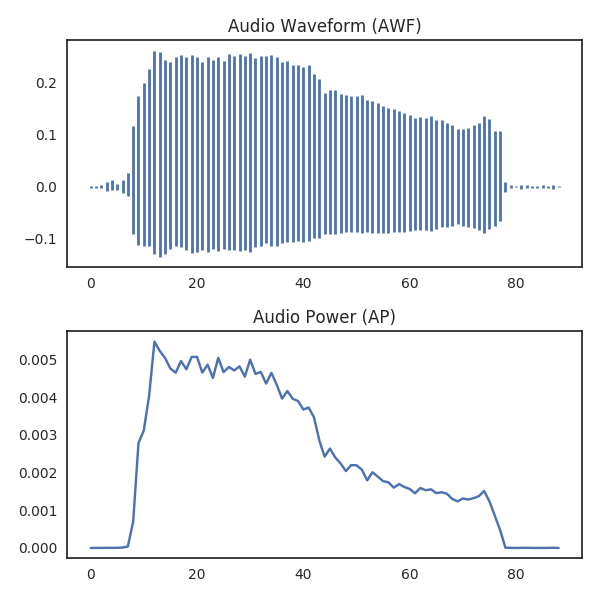
\includegraphics[width=\textwidth]{temporal-features-vertical.png}
        \end{figure}

        \column{0.5\textwidth}

        \begin{itemize}
            \item<2-> Log-Attack Time
            \item<3-> \textbf{Audio Waveform}
            \item<4-> \textbf{Audio Power}
            \item<5-> Temporal Centroid
            \item<6-> Effective Duration
            \item<7-> Auto-correlation
            \item<8-> Zero Crossing Rate
        \end{itemize}

    \end{columns}
\end{frame}

\begin{frame}
    \frametitle{Características espectrales}

    \begin{columns}
        \column{0.5\textwidth}

        \begin{figure}[!h]
            \centering
            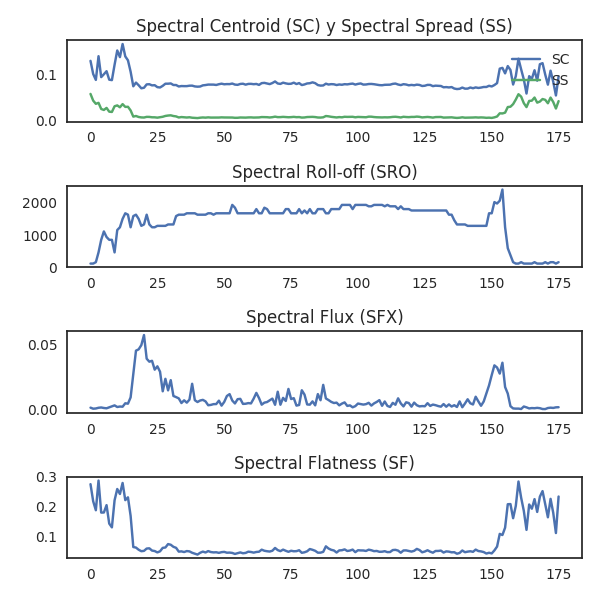
\includegraphics[width=\textwidth]{spectral-features-vertical.png}
        \end{figure}

        \column{0.5\textwidth}

        \begin{itemize}
            \item<2-> Frecuencia y amplitud picos
            \item<3-> Frecuencias mínima y máxima
            \item<4-> Bandwidth
            \item<5-> Cuartiles
            \item<6-> Spectral Shape:
            \begin{itemize}
                \item \textbf{Spectral Centroid}
                \item \textbf{Spectral Spread}
                \item \textbf{Spectral Roll-off}
            \end{itemize}
            \item<7-> \textbf{Spectral Flux}
            \item<8-> \textbf{Spectral Flatness}
        \end{itemize}

    \end{columns}
\end{frame}

\begin{frame}
    \frametitle{Características armónicas}

    \begin{columns}
        \column{0.5\textwidth}

        \begin{figure}[!h]
            \centering
            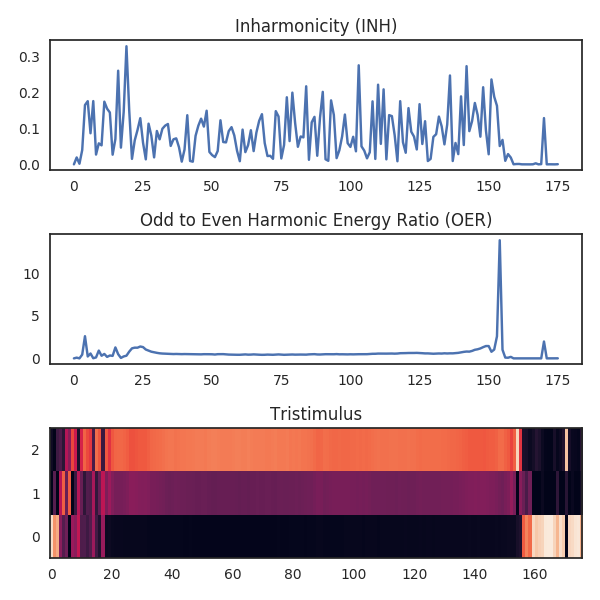
\includegraphics[width=\textwidth]{harmonic-features-vertical.png}
        \end{figure}

        \column{0.5\textwidth}

        \begin{itemize}
            \item Frecuencia Fundamental
            \item Picos armónicos
        \end{itemize}

        \begin{itemize}
            \item<2-> \textbf{Inharmonicity}
            \item<3-> \textbf{Odd to Even Harmonic Energy Ratio}
            \item<4-> \textbf{Tristimulus}
        \end{itemize}

    \end{columns}
\end{frame}

\begin{frame}
    \frametitle{Mel Frequency Cepstral Coefficients}

    \begin{columns}
        \column{0.5\textwidth}

        \begin{figure}[!h]
            \centering
            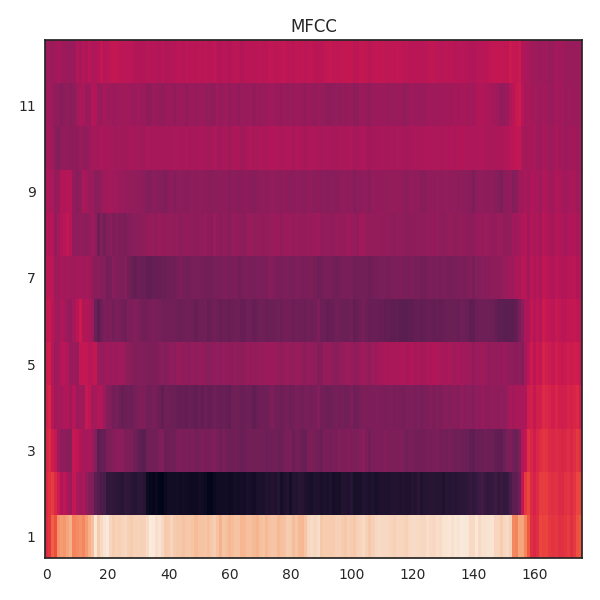
\includegraphics[width=\textwidth]{mfcc-square.png}
        \end{figure}

        \pause
        \column{0.5\textwidth}

        \begin{itemize}
            \item<2-> Caracterizar el contenido relevante de la señal, obviando características que aportan poca información.
            \begin{itemize}
                \item<3-> ruido de fondo
                \item<3-> emociones
                \item<3-> volumen
                \item<3-> tono
            \end{itemize}
            \item<4-> Desarrollada para el reconocimiento automático del habla humana.
        \end{itemize}

    \end{columns}
\end{frame}


